% Koma class
\documentclass[a4paper, oneside]{scrartcl}   

\usepackage{a4wide}

%------------------
% language = english
\usepackage[english, german]{babel}	% Umlaute mit \"u
\usepackage[latin1]{inputenc}

% margins + Kopf- und Fu�zeilen
\usepackage[left = 2.5cm, right = 2.5cm, top = 2cm, bottom = 3cm]{geometry}
\usepackage{scrpage2} 
\pagestyle{scrheadings}
\clearscrheadfoot
\rehead{\headmark}
\lehead{\pagemark}
\lohead{\headmark}
\rohead{\pagemark} 


% math
\usepackage{amssymb}
\usepackage{amsmath}

% figures
\usepackage{tikz}
\usepackage{graphicx}


% section-Zaehler wird neu gesetzt:
\setcounter{section}{3}
%------------------
\author{Sascha Meiers, Martin Seeger}
\title{Exercise 5, Discrete Mathematics for Bioinformatics}
\date{Winter term 2011/2012}


\begin{document}
\maketitle

%---------------------------------------------------------------------------------------------------

\subsection{Tree decomposition}

Let $G=(V,E)$ be a graph with $V= \{v_1 , \ldots, v_n\}$ and $E = {V \choose
2}$. We'll prove that the graph's tree width is $n-1$, meaning that any tree decomposition of $G$ 
contains at least one piece with $n$ elements.

\paragraph{Proof:} 
Given a tree decomposition $T$, let $V^*$ be the largest piece and assume that $v_n \notin V^*$ 
without loss of generality. We know by edge coverage property that there must be pieces containing 
$v_n$ and $v_i$ at the same time, for $1 \leq i \leq n-1$. Let these edges be covered by the $k$ pieces
$V_1, \ldots, V_k$ with $2 \leq k \leq n-1$ (but there could also be other pieces). $k$ cannot be one since 
then $V_k$ would be larger than $V^*$.

Now we analyze the structure of the tree $T$ and regard two cases:
\begin{enumerate}
\item The piece $V^*$ is somewhere ''between'' the pieces $V_i$.
        This means, there is at least one pair $(i,j)$ such that $V^*$ lies on a path from $V_i$ to $V_j$.
        $V_i$ and $V_j$ both contain $v_n$, but $V^*$ does not. This hurts the coherence property $\Rightarrow$ contradiction   
\item The piece $V^*$ is not between the pieces $V_i$. It could be a leaf of the tree, 
        but there could also be further pieces connected to it. However, $V^*$ is connected 
        to the subtree that contains all $V_i$ by a single edge.
        Let $X$ be the next piece on the path from $V^*$ to any $V_i$. 
        Usually\footnote{$X$ can contain at most $n-1$ nodes, so at least one node is missing, as stated. 
            Theoretically, the missing node could be $v_n$. But in this case, we have $X = V^*$ and 
            (if this is allowed at all) the argumentation (case 1 or 2) can be applied on $X$ itself as the largest set. }
        the piece $X$ is missing at least one node $v_l \neq v_n$. We know that there is at least one piece
        $V_r$ in the subtree that contains $v_l$, and we also know $v_l \in V^*$. By coherence property, 
        $X$ would also have to contain $v_l \Rightarrow$ contradiction.
        \begin{center}
        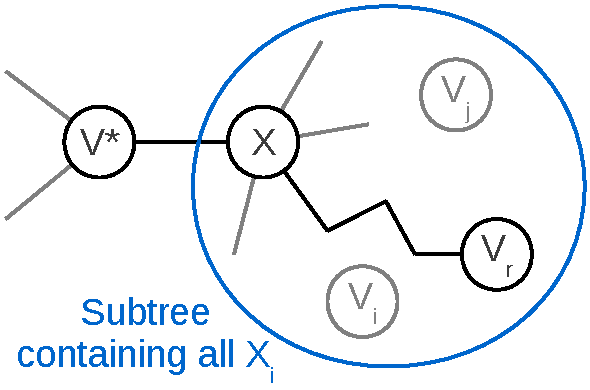
\includegraphics[width=6cm]{tree_decomposition_proof.pdf}
        \end{center}
\end{enumerate}


\subsection{Tree decomposition}


\subsection{Bellman-Ford}

\paragraph {a)}
\[ \begin{array}{c|ccccc}
   & z & u & v & x & y \\
   \hline
k=0 & (0)_z & \infty & \infty & \infty & \infty \\
k=1 & 0_z & 6_z & \infty & (7_z) & \infty \\
k=2 & 0_z & 6_u & (4_x) & 7_x & 2_u \\
k=3 & 0_z & (2_v) & 4_v & 7_x & 2_y \\
k=4 & 0_z & 2_u & 4_v & 7_x & (-2_u) \\
k=5 & (0_y) & 2_u & 4_v & 7_x & -2_y \\
\hline
\end{array} \]
Example: the shortest path from $z$ to $z$ is $(z,x,v,u,y,z)$ with weight zero (see traceback).



\paragraph {b)}
Let $f$ be the result of the Bellman-Ford-algorithm started in node $s$. We'll prove equivalency between the two statements (I) and (II):

\begin{description}
\item[(I)] The graph contains a circle of negative weight reachable from $s$.
\item[(II)] There is a node $v$ with $f_n(v) < f_{n-1}(v)$.

\item[(II) $\Rightarrow$ (I)] 
Let $v \neq s$ be the node for which we have $f_n(v) < f_{n-1}(v)$. 
By definition, $f_{n-1}(v)$ computed already the shortest walk $\pi^*$ 
from $s$ to $v$ using at most $n-1$ arcs. We say walk, because ensuring 
$\pi^*$ to be a path would require the graph not to contain negative circles.
But we consider $\pi^*$ to be a proper path, since if it was not we would
already have shown the implication.

So we assume $\pi^*$ is the shortest of all paths from $s$ to $v$, considering every 
possible path (since up to $n-1$ arcs suffice to cover every path). 
If $f_{n}(v) < l(\pi^*)$ then there is a new walk $\pi�$ that uses exactly $n$ 
arcs (if it used at most $n-1$ arcs, it would have been found in $f_{n-1})$.
A walk of $n$ arcs must contain a cycle $C$. And it contains a path from $s$ to $v$. 
Now the weight $l(\pi�)$ is made up of the 
weight of this cylce $C$ plus the weight of the path $\pi$ from $s$ to $v$ that is contained 
in $\pi�$ (Note that this decomposition need not be edge disjoint, but the edges that belong 
to the circle and the path at the same time are walked twice during $\pi�$, 
so the the addition of the lengths holds).    Now we have
\[ l(\pi�) < l(\pi*) \Rightarrow l(\pi�) < l(\pi) \Rightarrow l(\pi) + l(C) < l(\pi) \Rightarrow l(C) < 0 \]

\item[$\neg$(II) $\Rightarrow$ $\neg$(I)]
Now let us assume that there is no $v \in V$ such that $f_n(v) \neq f_{n-1}(v)$. Because trivially $f_n(v) \leq f_{n-1}(v)$,
this can only hold if $f_n(v) = f_{n-1}(v)$ $\forall v \in V$. 
However, as shown in the lecture,
\[
f_n(v) = \min (f_{n-1}(v), \min_{(u,v)\in A} (f_{n-1}(u)+l(u,v))).
\]
The second argument of the wrapping min function can therefore be not smaller than the first:
\[
f_{n-1}(v) \leq \min_{(u,v)\in A} (f_{n-1}(u)+l(u,v)) \hspace{3ex} \forall v \in V,
\]
or equivalently
\[
f_{n-1}(v) \leq f_{n-1}(u)+l(u,v) \hspace{3ex} \forall v \in V, (u,v)\in A.
\]

Now let $C$ be a cycle in the graph with $k$ different vertices $v_1, ..., v_k=v_0, v_{k+1}=v_1$. 
According to the previous inequality,
\[
f_{n-1}(v_i) \leq f_{n-1}(v_{i-1})+l(v_{i-1},v_i)
\]
is true for all $i$. Summing this inequality from $i=1$ to $k$, we obtain
\[
0 \leq \sum_{i=1}^k l(v_{i-1},v_i) = l(C).
\]
Since $C$ was any cycle in the graph, there are no negative cycles and our assertion follows.

\end{description}




\end{document}
